\documentclass[12pt]{article}
\usepackage[utf8]{inputenc}
\usepackage{upquote}
\usepackage[margin=1in]{geometry} 
\usepackage{amsmath,amsthm,amssymb}
\usepackage{graphicx}
\usepackage{listings}
\newenvironment{statement}[2][Statement]{\begin{trivlist}
\item[\hskip \labelsep {\bfseries #1}\hskip \labelsep {\bfseries #2.}]}{\end{trivlist}}
\usepackage{xcolor}




\title{Assignment 1}


\author{Author \\
  Wanjing Hu / fng685@alumni.ku.dk  \\
  Zhigao Yan / sxd343@alumni.ku.dk  \\
  Wanjing Hu / fng685@alumni.ku.dk  \\
  Wanjing Hu / fng685@alumni.ku.dk  \\
} 
 

\begin{document}
\maketitle


\section{26.1-1}
%wanjing
\textbf{Question: }Show that splitting an edge in a flow network yields an equivalent network. More formally, suppose that flow network $G$ contains edge $(u, v)$, and we create a new flow network $G'$ by creating a new vertex $x$ and replacing $(u, v)$ by new edges $(u, x)$ and $(x, v)$ with $c(u, x) = c(x, v) = c(u, v)$. Show that a maximum flow in $G'$ has the same value as a maximum flow in $G$.

\textbf{Answer: }As noted in the Question, we have $G'=(V',E')$ where $V'=V\cup{x}$, $E'=E-{(u,v)}\cup{(u,x), (v, x)}$.

First we should have a flow in $G'$ that is both a flow and a maximum flow. Construct $f'$ in $G'$ as follows:
\begin{equation}
f'(y,z) = 
\begin{cases}
f(y,z) &\mbox{if (y,z) $\neq$ (u,x) and (y,z) $\neq$ (x,v)}\\
f(u,v) &\mbox{if (y,z) = (u,x) or (y,z) = (x,v)}.
\end{cases}
\end{equation}
, where the $f$ is the maximum flow in $G$, and the only difference between $f$ and $f'$ is the $f(u,v)$ is replaced by two flows on the new added vertex $x$, valuing $f(u,v)$.

\subsection{Proof of flow - capability constraints}

According to the $c(u, x) = c(x, v) = c(u, v)$ in Question, we have:

\begin{gather}
f'(u,x) = f(u,v) <= c(u,v) = c(u,x)\\ \nonumber
f'(x,v) = f(u,v)<=c(u,v) = c(x,v)\\ \nonumber
f'(y,z) = f(y,z) <= c(y,z), when (y,z) \neq (u,x) and (y,z) \neq (x,v) \nonumber
\end{gather}

Also we have the $f'(y,z)>= 0$ for any $(y,z)$.

So the $f'$ we constructed obeys the flow capability constraints.

\subsection{Proof of flow - flow conservation}

Here we look at the flow going throw three vertex: $u$, $v$, and $x$. The rest of the vertex are naturally proved by $f$ is obeying the flow conservation. 

\textbf{Case $u$} Assume $u \notin \{s,t\} $, since $f$ obeys flow conservation, we can do as follows:

\begin{equation}
\begin{aligned}
\sum_{y \in V'} f'(u,y) &= \sum_{y \in V - \{x\}} f'(u,y) + f'(u,x)\\
&= \sum_{y \in V - \{v\}} f(u,y) + f(u,v)\\
&= \sum_{y \in V} f(u,y) \\
&= \sum_{y \in V} f(y,u) \\
&= \sum_{y \in V} f'(y,u) \\
\end{aligned}
\end{equation}

\textbf{Case $v$}
This is quite symmetric to the case $u$.
\begin{equation}
\begin{aligned}
\sum_{y \in V'} f'(y,v) &= \sum_{y \in V - \{x\}} f'(y,v) + f'(x,v)\\
&= \sum_{y \in V - \{u\}} f(y,v) + f(u,v)\\
&= \sum_{y \in V} f(y,v) \\
&= \sum_{y \in V} f(v,y) \\
&= \sum_{y \in V} f'(v,y) \\
\end{aligned}
\end{equation}

\textbf{Case $x$}

\begin{equation}
\begin{aligned}
\sum_{y \in V'} f'(y,x) &= f'(u,x)
&= f(u,v)
&= f'(x,v)
&= \sum_{y \in V'} f'(x,y)
\end{aligned}
\end{equation}


So the $f'$ we constructed obeys the flow flow conservation, and $f'$ is a valid flow.

\subsection{Proof of maximum flow}
Here we have two cases: one is $s \in \{u, v\}$ and the other is $s \notin \{u, v\}$. 

For the first case, we here prove the $s=u$ case since the $s=v$ case would be symmetric.
\begin{equation}
\begin{aligned}
 |f'| &= f_s\\
 &= \sum_{y \in V'} f'(u,y) - \sum_{y \in V'} f'(y,u) \\
 &= \sum_{y \in V'-{x}} f'(u,y) + f'(u,x) - \sum_{y \in V'} f'(y,u)\\
 &= \sum_{y \in V-{v}} f(u,y) + f(u,v) - \sum_{y \in V} f(y,u)\\
 &= \sum_{y \in V} f(u,y)  - \sum_{y \in V} f(y,u)\\
 &=|f|
\end{aligned}
 \end{equation}

For the second case, we have $x$ not connected to $s$ or $t$. Then we can prove as follows:
\begin{equation}
\begin{aligned}
 |f'| &= f_s\\
 &= \sum_{y \in V'} f'(s,y) - \sum_{y \in V'} f'(y,s) \\
 &= \sum_{y \in V-{x}} f'(s,y) + f'(s,x) - \sum_{y \in V-{x}} f'(y,s) - f'(x,s) \\
 &= \sum_{y \in V} f'(s,y) + 0 - \sum_{y \in V} f'(y,s) - 0 \\
 &= \sum_{y \in V} f(s,y) - \sum_{y \in V} f(y,s)  \\
 &= |f|
 \end{aligned}
 \end{equation}

As all above, the proof is done. We also notice that we did not make use of the feature that $f$ is a maximum flow in $G$, so for all the flows the $|f'| =|f|$ hold.

$Q.E.D.$
\section{26.1-4}
%wanjing
\textbf{Question: } Let $f$ be a flow network, and let $a$ be a real number. The scalar flow product denoted $af$, is a function from V x V to $\mathbb{R}$ defined by 

$(af)(u, v) = a \cdot f(u, v).$

Prove that the flows in a network form a convex set. That is, show that if $f_1$ and $f_2$ are flows, then so is $af_1+(1-a)f_2$ for all $a$ in the range $0<=a<=1$

\textbf{Answer:}

We are asked to prove that for all $0<=a<=1$, $af_1+(1-a)f_2$ satisfy both the flow conservation and the capacity constraint when $f_1$ and $f_2$ are valid flows. Let $G=(V,E)$ with $\{s, t\}$ and capability $c$, and $f1$, $f2$ are two flows in $G$.


\subsection{Proof of capability constraint}
First we prove the upper bound of the capability constraint:
\begin{equation}
\begin{aligned}
f'(u,v) &= (af_1)(u,v)+((1-a)f_2)(u,v) \\
 &= a \cdot f_1(u,v)+(1-a) \cdot  f_2(u,v) \\
 &<= a \cdot c(u,v)+(1-a) \cdot  c(u,v) \\
 &= c(u,v) \\
\end{aligned}
\end{equation}

Second we prove the lower bound of the capability constraint:
\begin{equation}
\begin{aligned}
f'(u,v) &= (af_1)(u,v)+((1-a)f_2)(u,v) \\
 &>= a \cdot 0+(1-a) \cdot 0 \\
 &= 0 \\
\end{aligned}
\end{equation}


\subsection{Proof of flow conservation}

For $f1$ and $f2$ we have;
\begin{equation}
\begin{aligned}
\sum_{y \in V} f_1(u,y) - \sum_{y \in V} f_1(y,u) &= 0 \\
\sum_{y \in V} f_2(u,y) - \sum_{y \in V} f_2(y,u) &= 0
\end{aligned}
\end{equation}


For $u \in V$, $u \notin \{s, t\}$: 
\begin{equation}
\begin{aligned}
&\sum_{y \in V} f'(u,y) - \sum_{y \in V} f'(y,u) \\
&= \sum_{y \in V} a \cdot f_1(u,y) + (1-a) \cdot f_2(u,y)  - \sum_{y \in V}  a \cdot f_1(y,u) + (1-a) \cdot f_2(y,u)\\ 
&= \sum_{y \in V} a \cdot f_1(u,y) + \sum_{y \in V}(1-a) \cdot f_2(u,y) - \sum_{y \in V}  a \cdot f_1(y,u) -  \sum_{y \in V}  (1-a) \cdot f_2(y,u)\\
&= \sum_{y \in V} a \cdot f_1(u,y)  - \sum_{y \in V}  a \cdot f_1(y,u) + \sum_{y \in V}(1-a) \cdot f_2(u,y) -  \sum_{y \in V}  (1-a) \cdot f_2(y,u)\\
&= 0 + 0\\
&= 0
\end{aligned}
\end{equation}

$Q.E.D.$

\section{26.1-7}

\section{26.2-2}
\section{26.2-4}
%zhigao
\begin{figure}[h]
    \centering
    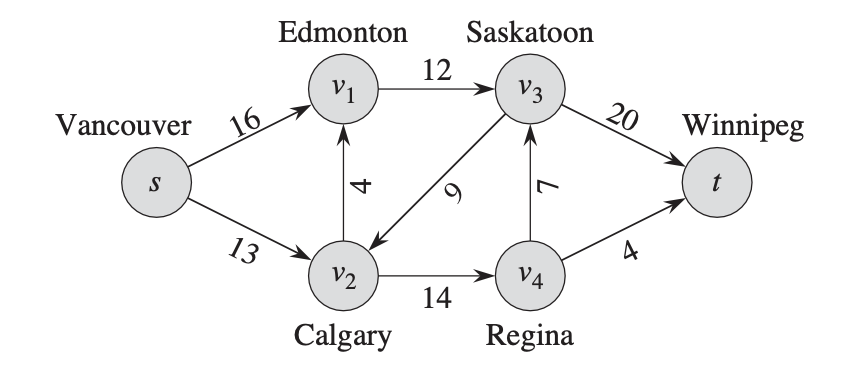
\includegraphics[width=0.5\linewidth]{截屏2024-11-18 下午8.43.56.png}
    \caption{26.1(a)}
    \label{fig:26.1(a)}
\end{figure}
By executing the Edmonds-Karp algorithm in 26.1(a), the first shortest path found is 
\[s \rightarrow v_1 \rightarrow v_3 \rightarrow t\]
The maximum flow on this path is 12.
Then updated the residual network:
\[s \rightarrow v1: 4, \quad v1 \rightarrow v3: 0, \quad v3 \rightarrow t: 8\]
\[v1 \rightarrow s: 12, \quad v3 \rightarrow v1: 12, \quad t \rightarrow v3: 12\]
Then use the updated residual network to find the next path:
\[s  \rightarrow v_2 \rightarrow v_4 \rightarrow t\]
The maximum flow on this path is 4.
Then updated the residual network:
\[s \rightarrow v2: 9, \quad v2 \rightarrow v4: 10, \quad v4 \rightarrow t: 0 \]
\[v2 \rightarrow s: 4, \quad v4 \rightarrow v2: 4, \quad t \rightarrow v4: 4 \]
Repeatedly, use the updated residual network to find the next path:
\[s \rightarrow v_2 \rightarrow v_4  \rightarrow v_3 \rightarrow t\]
The maximum flow on this path is 7.
Then updated the residual network:
\[s \rightarrow v2: 2, \quad v2 \rightarrow v4: 3, \quad v4 \rightarrow v3: 0 \quad v3 \rightarrow t: 1\]
\[v2 \rightarrow s: 11, \quad v4 \rightarrow v2: 11, \quad v3 \rightarrow v4: 7 \quad t \rightarrow v3: 19\]
At this point no other path can be found, so the total maximum flow is \(12+4+7=23\).
\section{26.2-3}
\begin{figure}[h]
    \centering
    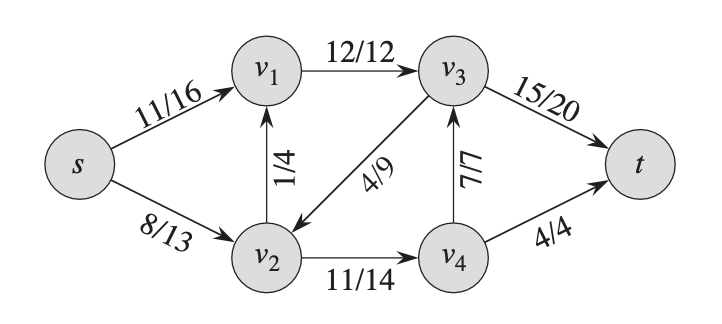
\includegraphics[width=0.5\linewidth]{截屏2024-11-18 下午8.46.37.png}
    \caption{26.1(b)}
    \label{fig:enter-label}

\end{figure}
Calculated in accordance with CLRS formulas 26.9 and 26.10.

\[f(S, T) = \sum_{u \in S} \sum_{v \in T} f(u, v) - \sum_{u \in S} \sum_{v \in T} f(v, u)\]
\[c(S, T) = \sum_{u \in S} \sum_{v \in T} c(u, v)\]

\[f(S, T) = f(s,v1)+f(v2,v1)+f(v4,v3)+f(v4,t) - f(v3,v2) = 11+1+7+4-4=19\]
\[c(S, T) = c(s,v1)+c(v2,v1)+c(v4,v3)+c(v4,t)=16+4+7+4=31\]
%zhigao
\section{26.2-7}
Firstly, I need to check the capacity constraint.\\
We know that : \(c_f(p) = \min \{ c_f(u, v) : (u, v) \text{ is on } p \}\)
Hence we have the following:
\[c_f(p) \leq c_f(u, v) \quad \forall (u, v) \in p.\]
So the capacity constraint is satisfied.\\
Then check the flow conservation.\\
We know the \(p\) is an augmenting path, And from the definition:
\[f_p(u, v) =
\begin{cases} 
c_f(p), & \text{if } (u, v) \text{ is on } p, \\ 
0, & \text{otherwise}.
\end{cases}\]
Assume that \(w\) is an output point and that \(w \in p\), Hence:
\[f_p(v, w) = c_f(p)\]
So we get: 
\[\sum_{u \in p} f_p(u, v) =\sum_{w \in p} f_p(v, w)\]
The flow conservation is satisfied.\\
By the definition of the augmenting path, the maximum amount by which we can increase the flow on each edge in an augmenting path is the residual capacity of \(p\).
So the flow on each edge is \(c_f(p)\), so \( |f_p| = c_f(p)> 0\)
%zhigao
\section{26.2-9}
\section{26.3-2}

\end{document}
